\section{Introduzione}

\subsection{L'azienda}
Il Gruppo Lynx è una realtà internazionale che opera nell'ambito della consulenza informatica. La consolidata expertise maturata in ambito tecnologico e di business, unitamente all'utilizzo di collaudate metodologie gestionali, consente a Lynx di proporsi ai propri Clienti come partner strategico per la realizzazione di progetti innovativi con soluzioni e know-how specifici. \\
Obiettivo principale di Lynx è continuare ad accrescere le proprie competenze funzionali e tecnologiche nei settori in cui opera, per offrire soluzioni efficaci che rispondano alle esigenze dei clienti. \\
Lynx è attiva in molti settori a livello internazionale, in particolare in quello dei servizi informatici nell'ambito della finanza, ma anche nel settore energetico e dei trasporti. \\

\begin{figure}[!ht]
	\centering
	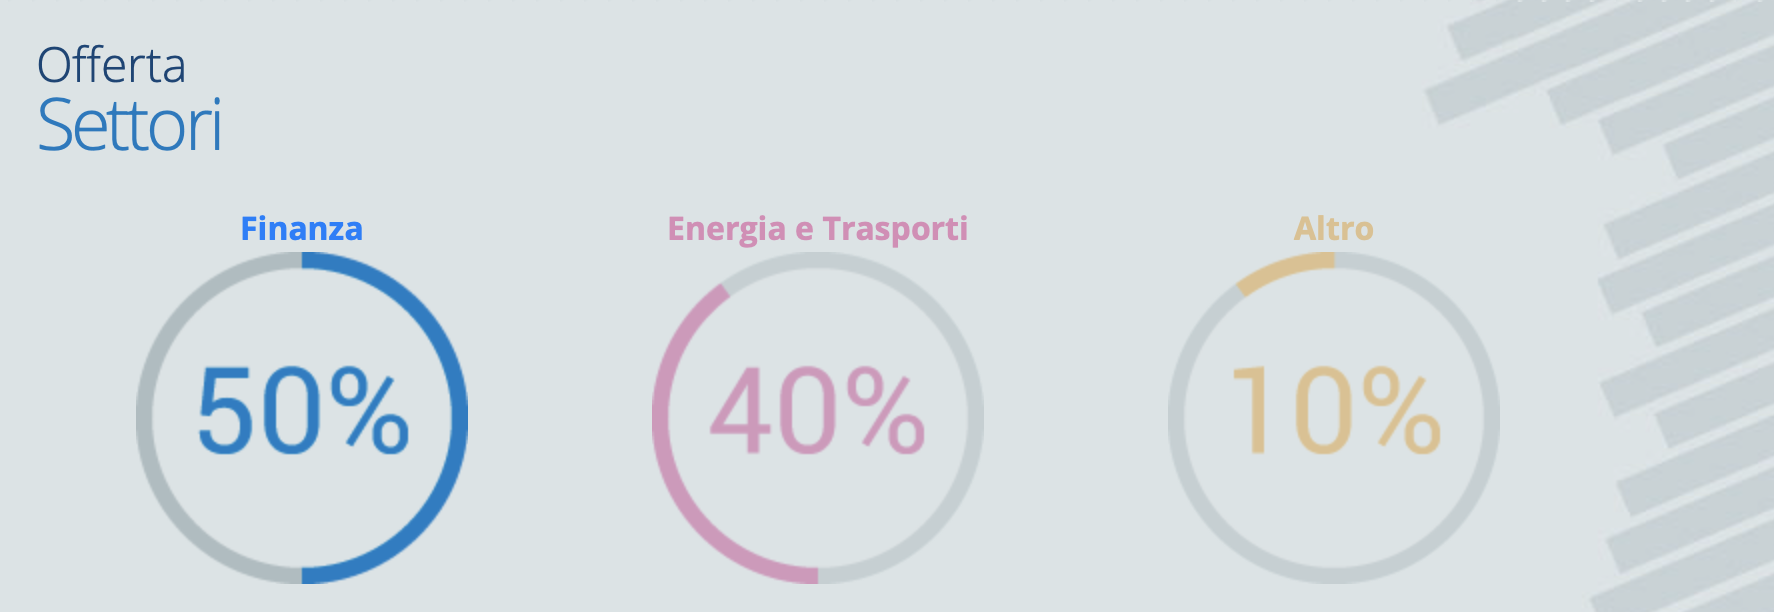
\includegraphics[width=0.6\textwidth]{./res/img/settori.png}
	\caption{Percentuali di aziende servite da Lynx nei vari settori.}
\end{figure}

\subsection{Intesa SanPaolo e Sportello}
\azienda collabora da anni con Intesa SanPaolo l'istituto bancario più grande del paese che conta moltissimi dipendenti. Tra i servizi offerti c'è l'applicazione che gestisce il workflow e i servizi all'interno delle filiali, denominata \textbf{Sportello}. \\
Lynx in collaborazione con Microsoft è stata chiamata a gestire il progetto di \textbf{Nuovo Sportello}. L'applicativo opera in tutte le filiali Intesa SanPaolo presenti sul territorio nazionale ed è utilizzato ogni giorno da migliaia di utenti. \\
Lynx offre a Intesa SanPaolo per Nuovo Sportello un servizio di AM (Assets Management) e uno di Evolutiva per lo sviluppo di nuove funzionalità. \\
La parte client del Nuovo Sportello è una web application basata su framework ASP.NET, utilizzabile su browser. Questo rende l'applicazione di facile utilizzo, versatile e molto più facile da mantenere. \\ 
In una sezione successiva descriverò in dettaglio la struttura e l'architettura del software. \\

\subsection{Ruoli e organizzazione aziendale}
Essendo Lynx una realtà molto estesa che conta molti dipendenti, durante il tirocinio sono riuscito a venire a contatto con poche persone, ma ho potuto farmi un'idea generale della sua organizzazione. Ogni macro-progetto con un cliente specificato, come ad esempio Sportello, è seguito da un buon numero di persone divise in team. Per quanto riguarda Sportello, si seguono molto i principi del modello Agile:
\begin{itemize}
	\item Soddisfazione del cliente, attraverso un consegna continua di software validato.
	\item Continuous Delivery (nel caso di sportello avviene un rilascio major ogni mese, che contiene bugfixing e nuove funzionalità)
	\item Continua iterazione e coperazione tra cliente, azienda e sviluppatori.
	\item Iterazione di tipo faccia a faccia tra persone.
	\item Ritmo sostenibile di sviluppo.
	\item Attenzione alla qualità del codice e al buon design.
\end{itemize}
Ho notato anche affinità con i principi del framework SCRUM, nella divisione in team, l'iterazione quotidiana e le scadenze.\\
Durante la mia esperienza di tirocinio ho avuto modo di far parte di due team diversi e vedere in generale il metodo di lavoro aziendale. 

\subsubsection{Gestione del telelavoro}
Durante la pandemia come moltissime altre aziende, Lynx ha aumentato il numero di ore e persone in telelavoro. Anche agli stagisti è capitata la stessa sorte. Tuttavia ho potuto constatare che il lavoro è ben organizzato, grazie alla lunga esperienza di Lynx nel settore.
La maggior parte del lavoro l'ho svolto da casa, con gli strumenti adatti. Ho potuto però notare la mancanza dell'iterazione fisica importante anche nel nostro settore, nel quale è fondamentale stringere relazioni.

\pagebreak